%%%%%%%%%%%%%%%%%%%%%%%%%%%%%%%%%%%%%%%%%
% Wenneker Article
% LaTeX Template
% Version 2.0 (28/2/17)
%
% This template was downloaded from:
% http://www.LaTeXTemplates.com
%
% Authors:
% Vel (vel@LaTeXTemplates.com)
% Frits Wenneker
%
% License:
% CC BY-NC-SA 3.0 (http://creativecommons.org/licenses/by-nc-sa/3.0/)
%
%%%%%%%%%%%%%%%%%%%%%%%%%%%%%%%%%%%%%%%%%

%----------------------------------------------------------------------------------------
%	PACKAGES AND OTHER DOCUMENT CONFIGURATIONS
%----------------------------------------------------------------------------------------

\documentclass[10pt, a4paper, twocolumn]{article} % 10pt font size (11 and 12 also possible), A4 paper (letterpaper for US letter) and two column layout (remove for one column)

\usepackage[hidelinks]{hyperref}
\usepackage{cleveref}
\usepackage{graphicx}
\usepackage{listings}
\usepackage{amssymb}
\usepackage{amsmath}
\usepackage{pifont}

\newcommand{\xmark}{\ding{55}}%
%%%%%%%%%%%%%%%%%%%%%%%%%%%%%%%%%%%%%%%%%
% Wenneker Article
% Structure Specification File
% Version 1.0 (28/2/17)
%
% This file originates from:
% http://www.LaTeXTemplates.com
%
% Authors:
% Frits Wenneker
% Vel (vel@LaTeXTemplates.com)
%
% License:
% CC BY-NC-SA 3.0 (http://creativecommons.org/licenses/by-nc-sa/3.0/)
%
%%%%%%%%%%%%%%%%%%%%%%%%%%%%%%%%%%%%%%%%%

%----------------------------------------------------------------------------------------
%	PACKAGES AND OTHER DOCUMENT CONFIGURATIONS
%----------------------------------------------------------------------------------------

\usepackage[english]{babel} % English language hyphenation

\usepackage{microtype} % Better typography

\usepackage{amsmath,amsfonts,amsthm} % Math packages for equations

\usepackage[svgnames]{xcolor} % Enabling colors by their 'svgnames'

\usepackage[hang, small, labelfont=bf, up, textfont=it]{caption} % Custom captions under/above tables and figures

\usepackage{booktabs} % Horizontal rules in tables

\usepackage{lastpage} % Used to determine the number of pages in the document (for "Page X of Total")

\usepackage{graphicx} % Required for adding images

\usepackage{enumitem} % Required for customising lists
\setlist{noitemsep} % Remove spacing between bullet/numbered list elements

\usepackage{sectsty} % Enables custom section titles
\allsectionsfont{\usefont{OT1}{phv}{b}{n}} % Change the font of all section commands (Helvetica)

%----------------------------------------------------------------------------------------
%	MARGINS AND SPACING
%----------------------------------------------------------------------------------------

\usepackage{geometry} % Required for adjusting page dimensions

\geometry{
	top=1cm, % Top margin
	bottom=1.5cm, % Bottom margin
	left=2cm, % Left margin
	right=2cm, % Right margin
	includehead, % Include space for a header
	includefoot, % Include space for a footer
	%showframe, % Uncomment to show how the type block is set on the page
}

\setlength{\columnsep}{7mm} % Column separation width

%----------------------------------------------------------------------------------------
%	FONTS
%----------------------------------------------------------------------------------------

\usepackage[T1]{fontenc} % Output font encoding for international characters
\usepackage[utf8]{inputenc} % Required for inputting international characters

\usepackage{XCharter} % Use the XCharter font

%----------------------------------------------------------------------------------------
%	HEADERS AND FOOTERS
%----------------------------------------------------------------------------------------

\usepackage{fancyhdr} % Needed to define custom headers/footers
\pagestyle{fancy} % Enables the custom headers/footers

\renewcommand{\headrulewidth}{0.0pt} % No header rule
\renewcommand{\footrulewidth}{0.4pt} % Thin footer rule

\renewcommand{\sectionmark}[1]{\markboth{#1}{}} % Removes the section number from the header when \leftmark is used

%\nouppercase\leftmark % Add this to one of the lines below if you want a section title in the header/footer

% Headers
\lhead{} % Left header
\chead{\textit{\thetitle}} % Center header - currently printing the article title
\rhead{} % Right header

% Footers
\lfoot{} % Left footer
\cfoot{} % Center footer
\rfoot{\footnotesize Page \thepage\ of \pageref{LastPage}} % Right footer, "Page 1 of 2"

\fancypagestyle{firstpage}{ % Page style for the first page with the title
	\fancyhf{}
	\renewcommand{\footrulewidth}{0pt} % Suppress footer rule
}

%----------------------------------------------------------------------------------------
%	TITLE SECTION
%----------------------------------------------------------------------------------------

\newcommand{\authorstyle}[1]{{\large\usefont{OT1}{phv}{b}{n}\color{DarkRed}#1}} % Authors style (Helvetica)

\newcommand{\institution}[1]{{\footnotesize\usefont{OT1}{phv}{m}{sl}\color{Black}#1}} % Institutions style (Helvetica)

\usepackage{titling} % Allows custom title configuration

\newcommand{\HorRule}{\color{DarkGoldenrod}\rule{\linewidth}{1pt}} % Defines the gold horizontal rule around the title

\pretitle{
	\vspace{-30pt} % Move the entire title section up
	\HorRule\vspace{0pt} % Horizontal rule before the title
	\fontsize{32}{36}\usefont{OT1}{phv}{b}{n}\selectfont % Helvetica
	\color{DarkRed} % Text colour for the title and author(s)
}

\posttitle{\par\vskip 15pt} % Whitespace under the title

\preauthor{} % Anything that will appear before \author is printed

\postauthor{ % Anything that will appear after \author is printed
	\vspace{10pt} % Space before the rule
	\par\HorRule % Horizontal rule after the title
	\vspace{10pt} % Space after the title section
}

%----------------------------------------------------------------------------------------
%	ABSTRACT
%----------------------------------------------------------------------------------------

\usepackage{lettrine} % Package to accentuate the first letter of the text (lettrine)
\usepackage{fix-cm}	% Fixes the height of the lettrine

\newcommand{\initial}[1]{ % Defines the command and style for the lettrine
	\lettrine[lines=3,findent=4pt,nindent=0pt]{% Lettrine takes up 3 lines, the text to the right of it is indented 4pt and further indenting of lines 2+ is stopped
		\color{DarkGoldenrod}% Lettrine colour
		{#1}% The letter
	}{}%
}

\usepackage{xstring} % Required for string manipulation

\newcommand{\lettrineabstract}[1]{
	\StrLeft{#1}{1}[\firstletter] % Capture the first letter of the abstract for the lettrine
	\initial{\firstletter}\textbf{\StrGobbleLeft{#1}{1}} % Print the abstract with the first letter as a lettrine and the rest in bold
}

%----------------------------------------------------------------------------------------
%	BIBLIOGRAPHY
%----------------------------------------------------------------------------------------

\usepackage[backend=bibtex,style=numeric,natbib=true]{biblatex} % Use the bibtex backend with the authoryear citation style (which resembles APA)

\addbibresource{refs.bib} % The filename of the bibliography
\DeclareNameAlias{default}{last-first}
\usepackage[autostyle=true]{csquotes} % Required to generate language-dependent quotes in the bibliography
 % Specifies the document structure and loads requires packages

%----------------------------------------------------------------------------------------
%	ARTICLE INFORMATION
%----------------------------------------------------------------------------------------

\title{The Botnet That Would Not Die} % The article title

\author{
	\authorstyle{Maximilian Hamminger, inf102409} % Authors
	\newline\newline % Space before institutions
	\institution{University of Applied Sciences Wedel, Wedel, Germany}\\ 
	\institution{Supervised by \textsc{Prof. Dr. Gerd Beuster} as part of the summer seminar 2019}\\ 
}

% Example of a one line author/institution relationship
%\author{\newauthor{John Marston} \newinstitution{Universidad Nacional Autónoma de México, Mexico City, Mexico}}

\date{\today} % Add a date here if you would like one to appear underneath the title block, use \today for the current date, leave empty for no date

%----------------------------------------------------------------------------------------

\begin{document}

\maketitle % Print the title

\thispagestyle{firstpage} % Apply the page style for the first page (no headers and footers)

%----------------------------------------------------------------------------------------
%	ABSTRACT
%----------------------------------------------------------------------------------------

\lettrineabstract{Botnets have been around for long---yet in most cases, law enforcement agencies or security researchers managed to take them down after all. In efforts to increase the resilience of their bots software, bot herders have developed new and better techniques to withstand attacks. When the bot herders realized that centralized botnets are easy targets, they switched to P2P botnets. As time has passed since the first observed P2P network, the current state of P2P networks has become highly resistant against most attacks. I provide an overview of the current situation, different variants of botnets and their weaknesses. In addition, I discuss the options we have against otherwise resilient botnets. }

%----------------------------------------------------------------------------------------
%	ARTICLE CONTENTS
%----------------------------------------------------------------------------------------

\begin{figure*}
		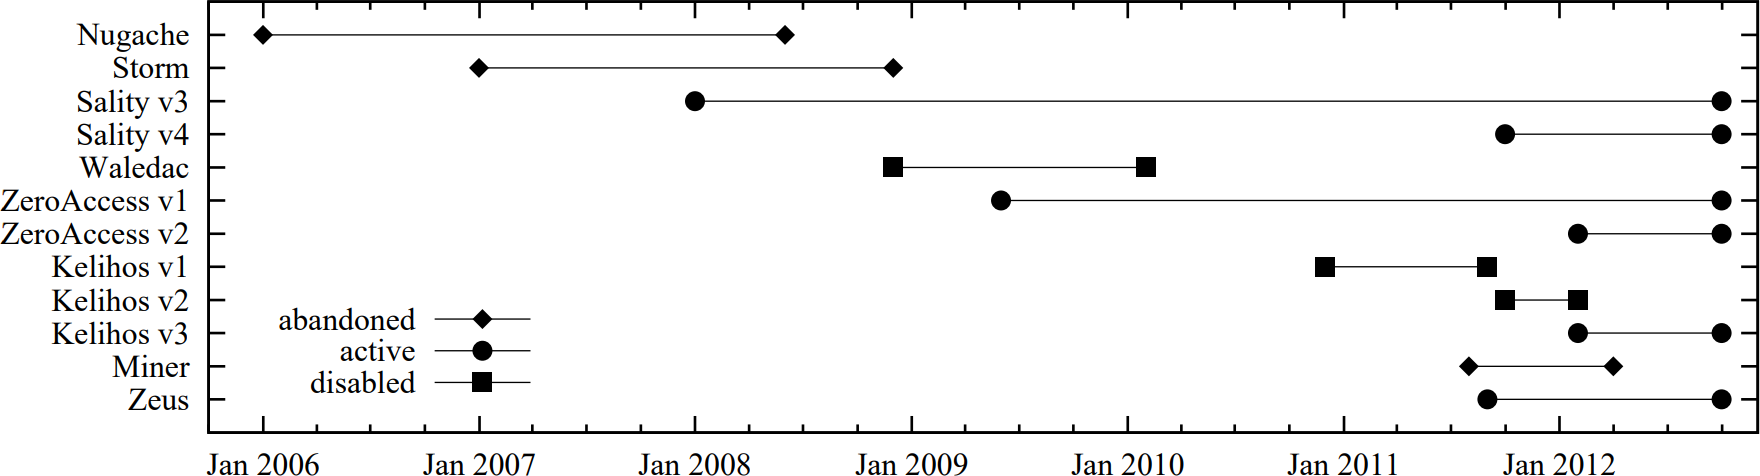
\includegraphics[width=\textwidth]{figures/lifetime.png}
		\caption{Lifetime of various botnets. Taken from the \citet{p2pwned}.}
\end{figure*}
\subsection*{Introduction}
This paper originated from my seminar work in the summer semester 2019 at the University of Applied Sciences Wedel, which was supervised by \textsc{Prof. Dr. Beuster}. It is about persistent botnets and the challenges we face in perspective to the ongoing developments in this field of cybersecurity. \\
A botnet is a network of devices, in which the participating clients (the bots) are infected by malware, allowing the attacker (the bot herder) to take over control of the device. Criminals often use botnets for various illegal activities, such as banking fraud, denial of service attacks or sending spam. Although most bot herders have criminal intentions, there are some speculations about state actors involved in certain botnets. As time progresses, botnets get more and more advanced and more resilient to the established takedown methods, making it harder for law enforcers to take them down. \\
I will start with a brief overview of well-known botnets and explain the difference between centralized and decentralized, peer-to-peer based botnets. Furthermore, I will show some methods which can be used for a takedown when the usual methods are not available and discuss their associated legal and ethical problems. This paper should offer a comprehensive overview of the challenges we face and how we could overcome these.

\tableofcontents
\pagebreak
\section{Motivation}

Before explaining the details of various kinds of botnets, I would like to present to you a famous botnet called GameOver ZeuS, which first attracted a lot of attention in September 2011 and stayed active until 2014, when a collaboration between the FBI, Europol, the British National Crime Agency and a few more private companies took down the botnet\cite{briankrebs}. ZeuS has caused losses that exceed \$100 million\cite{complaint}. \\
\\
Another example is Mirai: It was first seen in August 2016 by \textsc{MalwareTech} and caused massive DDoS attacks, which were reported as high as 1 Tbit/s\cite{goodin_2016}. 
\subsection{Example: GameOver ZeuS}
   GameOver ZeuS is a botnet, which is specialized in bank fraud. It was used to manipulate input fields in browsers to steal the banking data and generated huge losses. Apart from this, GameOver ZeuS was also used for the distribution of ransomware. In comparison to its predecessor, the ZeuS trojan, GameOver ZeuS depended on an encrypted peer-to-peer based communication for command and control and a domain generation algorithm(DGA for short) for a fallback channel. This made it quite hard for law enforcement to take down the botnet.
    
\subsection{Example: Mirai}
	Mirai however, is a different botnet than GameOver ZeuS: It is a centralized botnet, meaning it is relying on the direct communication with its Command \& Control server. It scanned the internet for insecure Internet of Things devices, like security cameras and routers, which used the default login data. When successful, Mirai would scan the device for competing malware and remove it when necessary. The next step is to contact the Command \& Control server and wait for any targets. The denial of service attacks from Mirai have been some of the largest and most disruptive ones\cite{mirai}. 
	
	\begin{figure}[ht]
		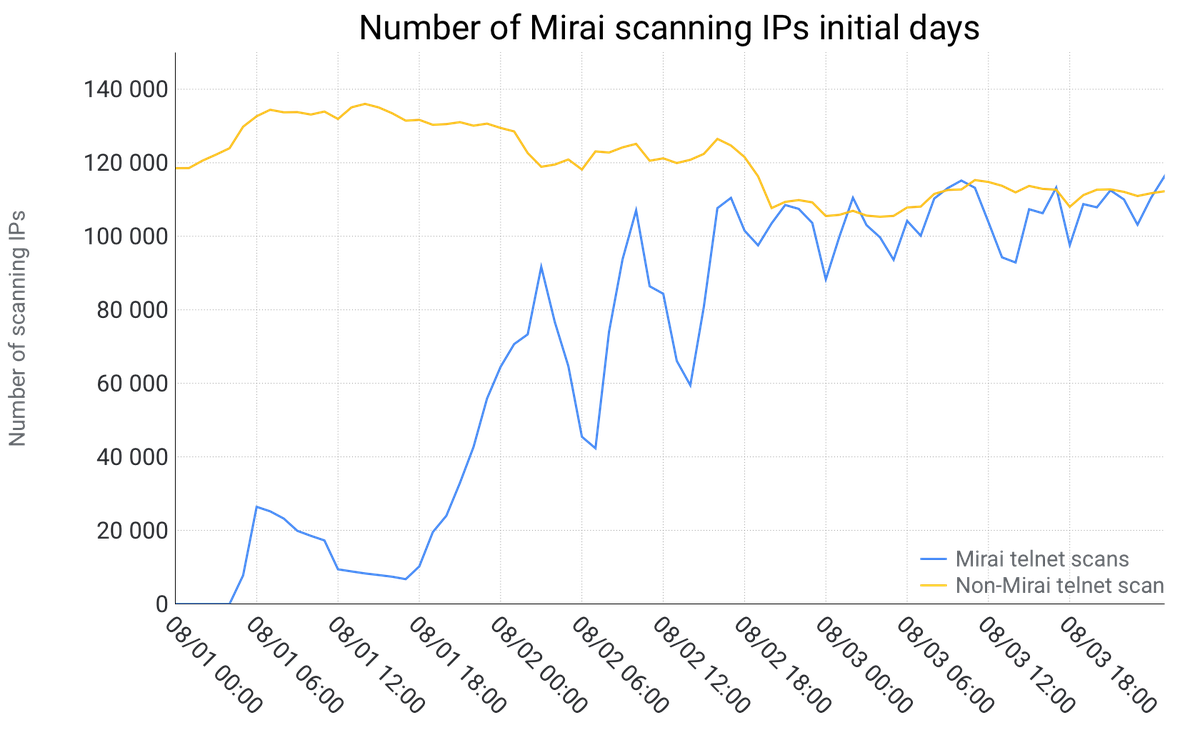
\includegraphics[width=\linewidth]{figures/mirai-initial-day-scanning-ips.png}
		\caption{Telnet scans from Mirai which were logged at cloudflares honeypots. Taken from \citet{cloudflare}. }
		\label{mirai}
    \end{figure}
	Another factor that made Mirai so successful was its quick growth, as can be seen in \autoref{mirai}. Mirai doubled its numbers in the early hours every 76 minutes\cite{cloudflare}.
\subsection{Problem description}
The problem that arises is the following: Botnets are becoming more and more harder to take down, as it can be seen with the ZeuS botnet, which needed a large joint venture operation. It needed the involvement of the FBI, Europol, and the British National Crime Agency, experts from the VU University Amsterdam, Saarland University; security firms, which were CrowdStrike, Dell SecureWorks, Symantec, TrendMicro and McAfee to be able to be taken down after 3 years of continues operation\cite{briankrebs}. The Sality botnet, however, was first seen in 2003 and due to still ongoing development, it is still online and operational. This is mainly due to its resilient design, which renders the traditional methods like sinkholing or shutting off a few servers useless. ``Hacking back'' is another option to take down a botnet, yet it is often not considered an option as it requires executing code on another person's device which is in many countries a criminal offense. In addition, it also raises a lot of ethical questions, which are discussed in \autoref{Legislature problems}.

\section{Centralized Botnets}
Most of the times in the past the creators of botnets went for a centralized network topology. In a centralized architecture, the bots try to contact a centralized command and control structure, which most of the times consists of one or a few command and control servers. A simplified model is shown in Figure 3:
\begin{figure}[ht]
  \centering
  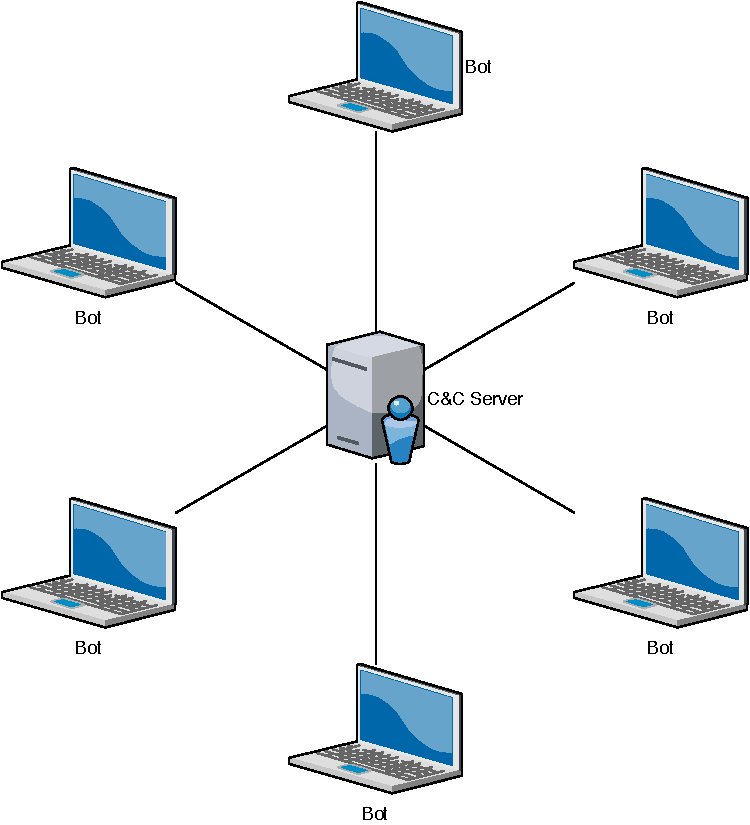
\includegraphics[width=\linewidth]{figures/central}
  \caption{Basic overview over the network topology of a centralized botnet.}
\end{figure} \\

Once the bots have successfully made contact with the command \& control server, the bots then await their actions. In many cases, the command \& control server is reachable under an IP address, which is either hardcoded into the bots software or obtained by a DNS lookup. However, there are a few ways to obfuscate the location of the command \& control server, as I will discuss in \autoref{hiding}. 
Centralized botnets can also be separated in two categories: Pull-based(for example, with HTTP) and push-based(as with IRC) communication. With pull-based communication, the bots check in a regular interval with the command \& control server for new commands, while with the push-based approach the bots remain in constant contact with the command \& control server and listen for new commands. 

\subsection{Architectural advantages and disadvantages}
From the attacker's point of view, the centralized architecture comes with a few advantages. To get a good understanding, why attackers still use this architecture instead of a more resilient one, I will list a few of the advantages here. 
\begin{description}
\item[Easy:]
The first advantage is that a centralized topology is relatively easy to implement and does not take that much time compared to a decentralized one. The attacker just needs his bots to connect to a server, which is often hosted on either hacked servers or from so-called ``bullet-proof hosters'', which promise to offer to host without having to worry about law enforcement, simply by not complying to court orders or moving the server to a different company if the external pressure gets too high. The actual programming effort is low. 
\item[Situation awareness:]
In addition, the attacker also knows fairly well about the current situation, as in how many bots are currently online, what their total network capability for denial of service attacks would be, who is behaving ``weird'', i.e. who might be doing research on his botnet. In many times, the bot herder will issue a denial of service attack against any non-complaint bots, meaning that researchers will have a slightly harder time to study the bot. There are a few differences here between pull-based and push-based ones: While push-based is quite accurate in its numbers since there is a constant connection between the command \& control server, pull-based communication can tend to be a bit off. 
\item[Efficiency:]
Furthermore, depending on the implementation details, a centralized botnet can be quite efficient. Take an IRC implementation for example, which is by design push based. A lot of bots can connect to an attacker-controlled IRC server and join a specific channel. Based on these channels, the bot herder knows how many are online and can by, for instance, setting the topic in the channel, send commands to all bots at the same time. Additionally, the bot herder can give commands to single bots at the time by the use of private messages. Another example would be a botnet which is HTTP based and therefore pull-based. Modern web servers can handle many thousand requests a second without problems\cite{nginx}, allowing for quick spreading of the botnet and low intervals between checks for new commands. 
\end{description}

Nevertheless, this architecture design comes with its own flaws and weaknesses. I will give a small summary of them here:
\begin{description}
\item[Single point of failure:]
By the nature of this design, it has a single point of failure: the command \& control infrastructure. Due to this, the bot herder needs to focus his main attention on methods to hide his Command \& Control infrastructure from the eyes of law enforcement agencies and other private researchers, as losing control over this part of the botnet means losing control over the whole botnet. Applicable methods for hiding this important part of the network are discussed in \autoref{hiding}. 
\item[Easy to track:]
Tracking a botnet means to gather intelligence about the metadata of the network. Often researchers want to know how many bots are active in the botnet, what the main purpose is and from where the infected devices originate. How this is done is often specific to the implementation details, e.g. when dealing with IRC based networks, the researchers can join the IRC server with the information contained in the bots software. Depending on the configuration of the server, the researchers can then see how many bots are online and what the commands from the bot herder are. In case this does not lead to any insights, the botnet can be tracked by another method at ISP level or by DNS providers. To determine the size of the botnet, the ISP can count the number of connections to the specific IP of the command \& control server. This can too be achieved over DNS, by counting the lookups for the corresponding DNS-Record, but it requires that the botnet uses DNS. Both methods however only deliver a small, regional insight into the actual network and can be overestimated due to changing IP addresses of the users. 
\item[Blocked easily:]
Another disadvantage from this type of design is that law enforcement agencies can use the single point of failure against the bot herder: By using the methods explained in \autoref{takedown}, the communication between the botnet and the command \& control infrastructure can be interrupted, thus leaving the bot herder without control and therefore without the ability to make money by blackmailing or different kinds of illegal activities.
Methods which can be used to block the control are among other things the following: 
\begin{itemize}
\item Sinkholing
\item Hosting provider de-peered
\item Hosting provider shuts off C\&C server
\item Exploitation of misconfigurations/bugs in the C\&C server
\end{itemize}
\end{description}
The details for these methods are explained in the following subsection, except for the Exploitation, as this is considered as an offensive option. However, we will discuss it eventually in \autoref{exploit}.


\subsection{Takedown Methods}\label{takedown}
To go into detail with each method for taking a server down, I have provided a list which explains the traditional methods of taking down a command \& control server. Moreover, I discuss what the problems with their application are.
\begin{description}

\item[Sinkholing:] \label{sinkhole}%WIKIPEDIA 
A DNS sinkhole is a DNS server, which is configured as such that each DNS query it receives, is checked against a blacklist. If the DNS query is on the blacklist, the DNS server then returns a fake address, redirecting the bot to a fake command \& control server (the sinkhole) in order to shut off communication with the bot herder. Sinkholes are also sometimes used to track and enumerate a botnet by counting the amount and type of requests. By design, a DNS server first checks in its cache if the request has already been requested, and if not, it will send the request to a higher-level DNS server. Consequently, the higher up the DNS server is in the DNS hierarchy, the more effective it is.\\
Another way to sinkhole a botnet is on the host-level. By editing the host file and adding the locations of the command \& control servers, one can redirect traffic to another address without having to change the DNS server.
\begin{figure}[ht]
  \centering
  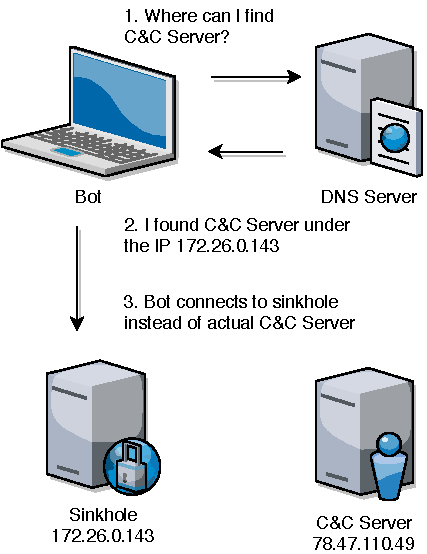
\includegraphics[width=\linewidth]{figures/sinkhole}
  \caption{Sinkhole concept}
\end{figure}

Yet it should be taken into account, that operating a sinkhole might mean that one will have to work with sensitive data, as the sinkhole will receive the data from the bots, which can feature functionality for identity theft or financial data, such as credit cards. 

\item[Physically shutting it off:]
This method makes the impression to be very straight forward. Shutting off the server or de-peering the hoster in case he does not cooperate sounds simple, requires however a few steps which are not so easy to accomplish. First of all, the location of the command \& control server needs to be known. We need to know the location of the server for two reasons: first, to shut it down and second, so we can get in touch with the local law enforcement. However, often a botnets command \& control infrastructure is spread through multiple countries. Furthermore, taking a botnet offline by shutting off the command \& control servers requires that these servers are shut off at the same time, otherwise, the bot herder can simply install new ones somewhere else. Since there are multiple countries involved, it also means there is a different jurisdiction in each country. This can be problematic, when one of the countries in which the server is hosted, decides to not cooperate. \\
Even when all countries cooperate, this method can still fail: Often times, ``bullet-proof'' hosters will try to evade law enforcement actions, by quickly moving the customer to a new hoster or simply refusing to work with law enforcement. In this situation, only a de-peering would work, as it happened in late 2008 with McColo. However, this does mean that not only law enforcement needs to cooperate, but also private firms who peered with the hoster. All in all, this is not an easy task.

\item[Cleanup of bots:]
Besides the other methods, a botnet can also be taken offline by removing the bots from the network, for example by removing the infections of the infected devices. On the other hand, this is easier said than done: the bots software has often certain functionality embedded, which disables installed antivirus software and is deeply integrated into the system to make removal hard. In addition to only removing the unwanted malware, the user has to update his device so that it will not be reinfected again. In case of the use of zero-days or usage of old software which is end of life and does not receive any updates anymore, like for example Windows XP, this is somewhat problematic.

\end{description}
It should be noted, that the first two methods do not completely solve the problem. In many cases, the bots are still active, however, fail to establish a connection to the command \& control server, as it is no longer reachable. This leads to the problem that the devices are still vulnerable and someone else might make use of this, by using backdoors or other mechanisms introduced with the initial infection. 


\subsection{Hiding the Command \& Control Server}\label{hiding}
To evade loss of control over the bots and therefore over the botnet, bot herders have developed over time a few different ways to hide their command \& control server. I provide an overview of the best-known ones here.
\pagebreak

\begin{description}
\item[Domain Generation Algorithms:] %WIKIPEDIA
Domain Generation Algorithms (in short: DGA) can be observed in various botnets. The DGAs can even differ in botnets themselves like it has been observed in GameOver ZeuS. Bitdefender reported that it has seen two variants in the wild: one of them generated 1000 domains a day, while another generated 10000 domains a day\cite{bitdefender}. These generated domains usually are used for ``rendezvous points'', meaning that for a certain time period a bot will be able to connect to a C\&C server under that address. Simply the huge amount of generated domains and also, when done correctly, the unpredictability of the algorithm's output makes it hard for law enforcement agencies to effectively shut down the connection between the bots and the C\&C server. \\
To make it harder for others to predict domains which the algorithm generates, DGAs often include external events, like trending topics on Twitter. \\
As an example, the bot herder would generate domain names using the same DGA as the one included in the bots and register only a few of them. The bots then would also generate their own list of domains, and try to contact a small portion of them in the effort of establishing communication with the C\&C server. \\
This technique gained its popularity by the Conficker worm, which first started with only 250 domain names a day, but was found to have increased the amount of generated domains to 50000 domains a day in later versions. Even despite the fact that it generates 50000 domains, it only tries to contact only 1 \% of them. If law enforcement would make an effort to sinkhole these domains---meaning to try to register each of these before the bot herder could, to redirect them to sinkhole---they would have to register 50000 domains per day. \\
There have been efforts to predict the domains generated by DGAs using machine learning, however, these can often be targets of adversarial techniques, which trick them into wrong results\cite{Sidi2019MaskDGAAB}. \\\\
An example for a domain generation algorithm can be seen here, which is written in python:

\begin{lstlisting}[language=python]
TLDS = [ '.com',
         '.biz', 
         '.us', 
         '.net', 
         '.org', 
         '.ws', 
         '.info']
DEFAULTTLD = ".in"
LETTERS = "asnhreqwpm" 

def dga(date, magic, number):
    year = date.year 
    month = date.month
    day = date.day 
    seed = year + month + day + magic
    r = Rand(seed)
    # for specified number of domains
    for i in range(1, number):
        # reset seed every 51 times
        if i == 51:
            r = Rand(magic)
        randomNumber = r.rand() 
        # array which is later
        # translated from indeces 
        # to letters
        ra = []
        # fill array with random 
        # numbers from 0 - 9
        for i in range(10):
            # append last digit 
            # from random number
            ra.append(randomNumber % 10) 
            # floor divide and assign
            randomNumber //= 10

        domain = ""
        # convert array of indeces
        # to a string, using indeces
        # to assemble from specified
        # letters array
        for x in ra:
            domain += LETTERS[x]
        # set tld. If first index 
        # in index array is higher than
        # the length of the tld array
        # then take the first one
        # else take the default
        if ra[0] < len(TLDS):
            tld = TLDS[ra[0]] 
        else:
            tld = DEFAULTTLD
        # append tld to domain
        domain += tld
        # return the domain
        # without jumping out 
        # of the function
        yield domain
\end{lstlisting}
This DGA was actually used in \textsc{MyDoom}, a computer-worm in 2004, so credits go to whoever the respective author is. It should be noted, that the random generator got modified as to such that it always returns a number which is at least 9 digits long. The full code can be found in a GitHub repo\cite{baderj}.  I have added comments and simplified it a bit to explain what it does for non-python users.
\pagebreak
\item[Flux:] %WIKIPEDIA and ENISA
Many botnets have used fast flux as a technique to increase their resilience against takedowns by hiding the exact location of their command \& control server. For example, the Storm and Rustock botnets used fast flux. The general idea is mostly the same as with content delivery networks\cite{Holz_measuringand}. 
\begin{figure}[ht]
  \centering
  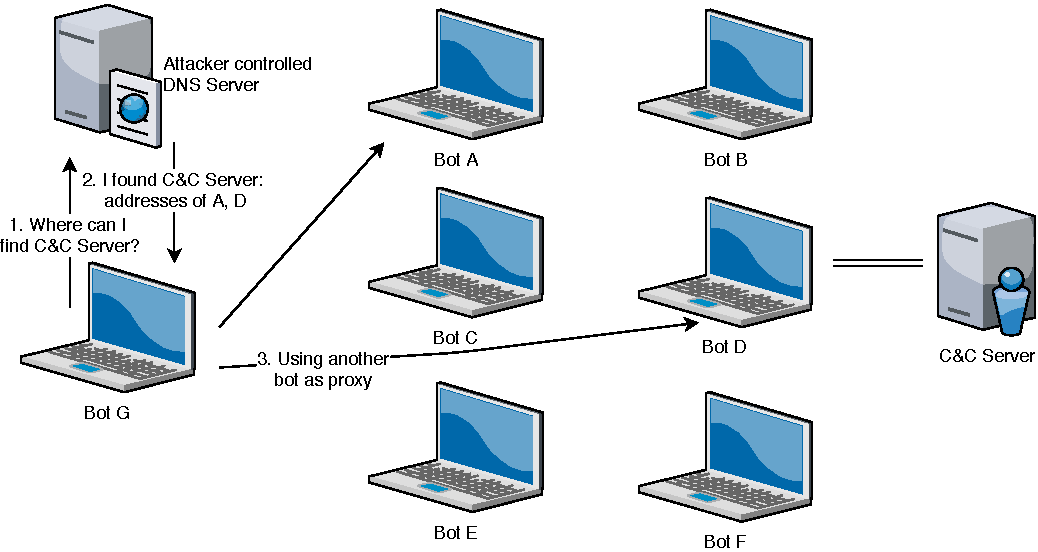
\includegraphics[width=\linewidth]{figures/flux}
  \caption{Fast Flux Network}
\end{figure}

When the bot queries his DNS server for the domain under which he tries to contact the command \& control server, the request is first sent to the nearest DNS server and is then forwarded to the bot herders DNS server. The bot herders DNS server will then answer with usually a large number of IP addresses, which all have a very short time to live, under which the bot can reach the command \& control server. These IPs commonly are associated with other bots in the network, which act as proxies to the actual command \& control server. The proxies will then forward all traffic to the command \& control server. Due to the very short time to live entries in the response from the DNS server, this will cause the results to be different each time the same domain is queried. 

\item[Tor:]
Tor, as an anonymous communication network, offers a service called ``Hidden Service''. It was added in 2004 and allows users to run a server anonymously over the Tor network. Tor itself works by providing another network, which uses ``Onion routing''. Onion Routing is done by encrypting the packet multiple times, however, with each encryption step, a destination IP of a randomly selected tor relay is added. By design, the packets get routed multiple times over these Tor relays, which can only decrypt the first layer to find out what the next destination for the packet is. When the packet arrives at its final relay, it will get decrypted by the relay, which then sends the original data to its actual destination. The important aspect in this is, that the last relay does not know who the original sender was, thus allowing for anonymity in the network---in this case, the hidden command \& control server which is implemented as a hidden service.\\
Using Tor for communication with the command \& control server also offers another advantage for the bot herder: he does not have to worry about NAT and Firewalls, as the communication goes directly through Tor. Furthermore, the bot herder can easily generate new .onion domains by generating new public keys\cite{defcon18}. \\
Due to the implementation of the Tor network, locating the command \& control server is often only possible by finding information leaks, such as a web server which reports its actual IP or exploiting the service by finding misconfigurations or bugs.

\end{description}

\section{P2P Botnets}
Peer-to-Peer Botnets, or decentralized Botnets, are botnets who do not need a central command \& control server. Instead, the bots enable communication within the botnet by peering with other bots\cite{enisa}. The corresponding network topology is called peer-to-peer (in short P2P), hence the name. Each bot knows only about a small subset of the botnet, which is known as peers for the bot. These peers are typically saved in a peerlist, which saves the addresses of the other bots. The bot can then talk to its peers to propagate new updates or commands, who then themselves talk to their peers, thus allowing for the spread of information and commands through the whole botnet. \\
In case of the first, the bots exchange when peering their version number, and if one revision is lower than the other, the older bot is updated to the newer version. Inserting new versions and/or commands can be done from any arbitrary point imaginable, making it hard to localize the origin. This process is slower than when realized in a centralized architecture, however, it comes with the great advantage of staying anonymous as a bot herder. In many cases, the bot herder uses code signing to prevent others from taking the botnet over. Famous examples of these decentralized botnets are the Storm worm, Nugache, and Conficker. 
\begin{figure}[ht]
  \centering
  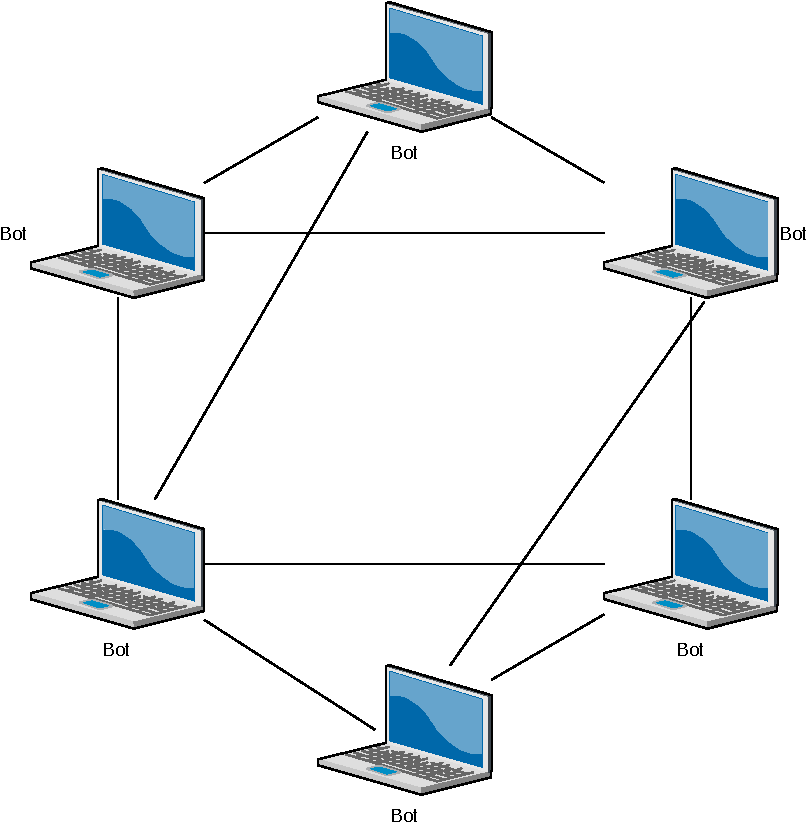
\includegraphics[width=\linewidth]{figures/p2p}
  \caption{Simplified version of an unstructured P2P network, where each bot has 3 other peers with whom he can talk.}
\end{figure} \\
Furthermore, P2P networks can be split into two categories: Unstructured and structured. Unstructured networks do not impose any particular structure for the network topology by design, but rather form by random connecting to other bots. Since there is no structure, communication between bots works by gossiping. Gossiping means that in order to find something, the bot has to inform all other bots, causing the network to be flooded with the search query. This usually means higher utilization of system resources, such as CPU and bandwidth. In addition, because the role of all peers is the same, the network is highly robust against high churn---that is, when a large number of bots enter and leave the network frequently. Most current botnets use this approach, such as Sality and Nugache.\\

Structured P2P networks, however, create in addition an overlay for efficient routing and searching in the network. Distributed hash tables are often the variant of choice for implementing efficient search methods, in which a variant of hashing is used to assign ownership of a certain file to a particular bot. A bot who would like to retrieve the file would then go on and look up in the distributed hash table the location of the file, and then contact the corresponding bot. The use of distributed hash tables, however, makes them less robust in situations where there is a high churn. One botnet which used a structured protocol is Storm.
\begin{figure}[ht]
  \centering
  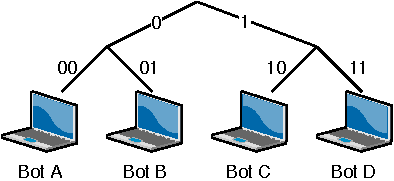
\includegraphics[width=\linewidth]{figures/structured}
  \caption{Structure of a structured P2P network, using distributed hash tables to identify and locate nodes.}
\end{figure}
\pagebreak
\subsection{Architectural advantages and disadvantages}
While P2P networks are designed to be highly robust against takedown attempts, they too suffer from some design flaws. Again, I will list and discuss the most prominent advantages and disadvantages.
\begin{description}
\item[Resilient by design:]
Many P2P botnets incorporate certain features, that make them highly resilient. However, some are also a result of the P2P architecture. The probably biggest advantages of P2P networks is that they do not feature a single point of failure, as with centralized botnets. Where in centralized botnets a central server sends out the commands and is critical for the botnet, P2P botnets use gossiping or an overlay for communication, as explained in the previous section. Furthermore modern P2P are harder to track, as the bots often do not use explicit identifiers and in addition, do not exchange peers often. Traditional methods like message spoofing also seem to lose their effectiveness: many networks today use encryption, preventing the commands from getting spoofed. I will talk more about these features in \autoref{resiliency}.

\item[Slow:]
One big disadvantage from P2P networks is, that they are comparably slow and inefficient in their communication and execution of commands. In unstructured networks, the message floods each time the network, which reduces efficiency. While structured networks do not suffer from this problem, as the message exchange can be realized efficient by targeting each bot just once, they too can not reach the quick reaction times a centralized, push-based network can reach. When they are by design pull-based, using the distributed hash table as a place to propagate new commands, they risk introducing a new single point of failure. Due to this, they need to include the same information at multiple locations. In addition, pull-based also means that the reaction time is still the maximum waiting time for a new pull command.   
\item[Harder to implement:]
While centralized botnets are relatively easy to get up and running, P2P networks need more knowledge about their individual advantages and disadvantages. To get a truly resilient, a lot has to be into consideration as the bot herder: How should I protect against message spoofing? How can I stop someone from partitioning my network? Do I structure my network, and if so, make myself vulnerable against index poisoning attacks? How do I deal with new bots, how can I make sure that they are legitimate and not a fake version from researchers or law enforcement?\\\\
In many cases, the bot herders design a custom protocol for these reasons, as for example the Storm botnet has shown that using already existing, filesharing P2P protocols are flawed when used for botnets.
\end{description}


\subsection{Resilience of P2P Networks}\label{resiliency} %P2k0wned
I am basing this subsection mainly on the paper ``P2PWNED — Modeling and Evaluating the Resilience of Peer-to-Peer Botnets'' by \citet{p2pwned}, who developed a graph-theoretical model to analyze current and future botnets in regard to resilience. The graph model itself is not part of this subsection, however, I will talk about the aspects of resilience featured in that paper.\\
First of all, Rossow et al. defined two aspects when it comes to resilience: 
\begin{description}
\item[Intelligence gathering resilience:] The more the bot can deter malware analysts from enumerating the botnet, the higher its resilience against gathering intelligence is. This is important, as we need to know the topology of the network and who is infected to figure out what attacks on P2P networks, and also what techniques for the mitigation, are even feasible. 

\item[Disruption resilience:] Secondly, another important aspect is how capable the network is against attacks from researchers and law enforcement agencies. Examples of disruption techniques include Sinkholing, which is explained under \autoref{sinkhole} or partitioning.
\end{description}
Another important point is, that these aspects do not apply to just one, very specific botnet, but instead to the general concept of P2P networks. This, however, does not mean that all techniques featured in this section will always work---as a matter of fact, most highly advanced botnets feature certain procedures to prevent this---but it should give a good starting point for starting research about a specific botnet, which then can be defeated using implementation-specific weak-points.

\subsubsection{Intelligence gathering resilience}
When it comes to gathering intelligence over a certain botnet, we can decide whether we want to do it actively (by crawling) or passively (by inserting probes). On a side note: Probes are also often called sensors.
\begin{description}
\item[Crawling:] Crawling is a known technique. To enumerate the botnet, simply visit every botnet and increment a counter by one. To further gain knowledge about the botnet, any other information which is provided by the bot should also be collected additionally. For example: Revision numbers, the version of the operating system, the current local time. However, this is specific to every communication protocol---not every protocol includes this information. Furthermore, many bot herders have made it hard to ``simply'' enumerate the bots, for instance, many bots do not use explicit identifiers, making it difficult to determine whether or not a bot has already been counted. In addition, there are many bots hiding behind firewalls or NAT, which means that they will not be reachable from the internet. Moreover, the network changes while crawling due to churn, limiting crawling to a certain time frame\cite{defcon21}. Since all of this also depends on the protocol, an exact amount can not be estimated. As a famous example, the Storm botnet has been estimated to contain more than a million bots, however, when it was taken down, the researchers only counted about 280k bots\cite{storm}. 
\end{description}

\begin{figure}[ht]
   \begin{lstlisting}[language=python]
def crawl():
    visitedPeers = []
    # initial seed peer list
    # obtained by random scanning
    # or decompiling the bot
    peerList = [A, B, C]
    while True:
        for bot in peerList:
            # only explore not 
            # yet visited bots
            if bot not in visitedPeers:
                cache = requestPeers(bot)
                # adds the requested 
                # peers to the 
                # peerList which has
                # yet to be visited
                peerList.extend(cache)
                # removes the  
                # bot itself 
                # the peerlist,
                #  avoiding cycles
                peerList.remove(bot)
                # finally add to 
                # visited peers
                visitedPeers.append(bot)
    \end{lstlisting} 
    \caption{A basic crawling algorithm in pseudo-python. It is an adapted version from \citet{p2pwned} P2P Botnet Graph Search algorithm. The size can be estimated using the size of the visited peers list.}
\end{figure}

\begin{description}
\item[Probes:] In contrast, when it is more important to gain knowledge about the peers instead of the topology of the network, another method can be used: Probes. This idea originating from \citet{kang} and was further generalized by \citet{p2pwned}. The basic idea is simple: Insert into the network special bots---probes---, which participate in the network. Inserting the probe into the network can be achieved by injecting the probe's address into the peerlist of other bots. As the other bots frequently need to check if the entry in their peer list is still online and responding as part of their peerlist verification, they have to communicate with the probe. This then can be used to enumerate the bots. Another advantage is that non-reachable bots can too be enumerated, as NATs and firewalls do not impose a problem. 
Nevertheless is the coverage of the probe highly depended on the amount of its address in other bots peerlist. To boost the coverage, the network can be crawled, inserting the probe into every crawled bot's peerlist. In some implementations of botnets, the probe would then also spread into not crawled bots by the exchange of peerlists between the participants in the network. 
However, this is a greatly specific to the implementation of the P2P botnet---In some, the probe has to continuously advertise itself in order to not prevent the removal of its address from the peerlist, while it other it does not. 
\end{description}

\begin{table}[h]
    \resizebox{\linewidth}{!}{%
    \begin{tabular}{@{}l|ccccc@{}}
        \toprule
        Botnet  & IDs & Invalid peers & \#  & Preference & Timeframe  \\ \midrule
        Kelihos & \checkmark & \xmark        & 250                       & Recent     & 10 minutes \\
        Nugache & \xmark     & \xmark        & 100                       & Recent     & Random     \\
        Sality  & \xmark     & \xmark        & 1                         & Random     & 40 minutes \\
        Storm   & \checkmark & \checkmark    & 10                        & Distance   & 10 minutes \\
        ZeuS    & \checkmark & \checkmark    & 10                        & Distance   & 30 minutes \\ \bottomrule
    \end{tabular}%
    }
    \caption{Overview over the most prominent P2P networks and their characteristics. \textit{IDs} is checked when the botnet uses unique IDs. \textit{Invalid peers} defines whether or not it is possible to include not routable peers in the peerlist. \textit{\#} stands for the maximum amount of peers exchanged and \textit{Preference} lists the criteria which decides which peer is choosen. \textit{Timeframe} is the interval between peer exchanges. Credits go to \citet{p2pwned}. }
\end{table}
Modern botnet creators, however, spend a considerable amount of time in order to make sure that they are not vulnerable to these techniques. In many cases, the exchange of peers is not frequent. In addition, the number of peers exchanged is often very low. Sality for example only exchanges one peer at a time every 40 minutes.



\subsubsection{Disruption resilience}\label{disruptRes}
In many cases tracking the development and trying to gain intelligence about the topology of the network and its bots, is only the first step. Knowing how many bots are currently active and what their metadata is, does not yet take the botnet down. A solution to bringing a network down on the infrastructure layer could be to partition or sinkhole it. On the communication layer, it is sometimes possible to use command poisoning, which is explained in detail in \autoref{sybil}. 

\begin{description}
\item[Partitioning:] Prohibiting the spread of commands and other information across the network results in a partitioned network, where one subset of the network is not able to communicate with the other. It is often the case after a successful analysis of the botnet, in which certain nodes---often so-called ``hot spots''---can be identified as the sources of new commands. This can be done by inserting unreachable or non-routable entries into the peerlist of this node, thus eliminating the possibility of that bot to send further commands. Usually, this is known as destroying the (bots) peerlist. Which bot would need it's peerlist destroyed depends on the structure of the botnet: In pull-based networks, one would eliminate the peerlist of the bots which pull from the central bot. In push-based networks, the one who is pushing the information would be the target. \\
This method nonetheless requires extensive knowledge about the topology of the network. For example, the hot spots need to be known and also who is peering with them.

\item[Sinkhole:] The general idea of a sinkhole is already explained in \autoref{sinkhole}. Thus I am concentrating in this part on sinkholing P2P networks, which basically transforms these into a central network. In this attack, all peers of each participating bot in the network are replaced by the address of the specific sinkhole, so that every bot knows at least one sinkhole but no other routable bot. When the sinkhole actively searches the botnet for other peers and their connection, it can furthermore announce itself to these bots. \\
In most cases, the sinkhole needs to exchange P2P messages (and due to this, implement at least a few of the protocol's mechanisms) to retain its popularity in the network, as becoming removed from the peerlist would render the sinkhole useless. 
In addition, inserting the sinkhole in all bots while also removing any routable peers is something which needs a lot of planning in advance and is not easily feasible.
\end{description}

Both attacks, sinkholing and partitioning, require that we can poison other peers peer list. Yet this is often not possible in the wild: For example, Sality in addition to one exchanging one peer every 40 minutes, also only replaces peers with a low reputation. Moreover, it picks these peers at random, unlike Nugache, which picks peers which are recent or Storm and ZeuS, which pick peers that are close by. Kelihos features a fast-flux channel for recovery, in cases where the P2P network is getting compromised. ZeuS, in addition, has a DGA-based recovery channel, which also allows for removing suspicious bots from the peerlist. 

\section{Options against P2P Botnets}
Every P2P botnet has to manage two important aspects: Keeping connectivity up and the exchange of information by routing. When a new bot joins the network, it needs a certain way to integrate itself in it. Typically this is achieved by exchanging peerlists and very often, this is the attack vector as it was with the attacks featured in \autoref{disruptRes} and \autoref{sybil}. \\

Nevertheless, there is another option which can be used against P2P-, but also against centralized-botnets, where it is not necessary to exploit the peerlist exchange procedure. It is often called \textit{poisoned fruit}.\\

\citet{proactive} categorized the different attack strategies in three different categories: \textit{Manipulation}, \textit{Mitigation} and \textit{Exploitation}. I will explain what defines the categories in each corresponding section. 
\subsection{Reducing effectivity of P2P Networks}
Instead of taking the botnet down, the general idea is to reduce the effectiveness of the network for the bot herder by such an amount, that it becomes uninteresting to further maintain it. Since this requires knowledge and the use of the communication protocol of the specific botnet, this is can be categorized as manipulation.\\ 
\begin{description}
\item[Poisoned fruit:] The poisoned fruit idea explores this concept: It bases on injecting wrong, sometimes even traceable datasets into the network.\\ 
An example: A botnet is specialized in stealing credit cards. After the device has been infected, the bot will constantly monitor the machine for new credit card data, and when it registers new entries, it will report the credit card data to the network, from which the bot herder then collects the entries and sells them on the black market.\\
Applying the concept to this network would mean that we would start by inserting a few bots which can be controlled into the network. After the bots have been deployed, we would then go on and start sending out fake credit cards, which have been registered(as in, saved for later identification). \\
This reduces the effectiveness of the network proportional to the percentage of inserted fake data to the overall amount of data harvested in a given timeframe, as the fake credits card do not work and thus cannot be sold. It also damages the reputation from the bot herder on the black market, as an increased amount of not working credit card numbers will be provided to buyers. This will force the bot herder to either stop selling credit cards or having to test each harvested credit card number, which will increase the time and effort needed for an effective botnet used for fraud. \\
In this example lies another advantage: As the inserted credit cards have been registered before it was inserted into the network, they can later be identified. As a result, the botnet can later in ongoing law enforcement efforts linked to certain sellers. A similar approach as with registered banknotes in the case of a abduction with a ransom demand.\\\\

\item[Index Poisoning Attack:] In an index poisoning attack a malicious bot spams the distributed hash table with false locations\cite{indexattack-def}, often by adding entries which do not hold the information, therefore forcing the bot to try another location for fetching the file. The larger the amount of inserted false index information, the less effective is fetching the file. \\
As shown in \autoref{indexpoison}, when a bot wants to publish a piece of information, such as commands or an update file, it will add an entry to the DHT, allowing others to query for it. In the next step, the attacker then adds entries for that information to the DHT, however with locations which are not reachable. When a bot then wants to obtain the information, it queries the DHT, which will respond with the location of the file. As the attacker has already inserted bogus information, chances are that the bot will receive a not reachable location or a location, which simply does not possess that information. This results in the querying bot wasting a great amount of time contacting peers which either do not respond or do not possess the information. Research from \citet{indexattack} has shown that on certain P2P networks, such an attack can reduce the ability to successfully download a piece of information to 0.004\%.  

\end{description}
\begin{figure}[ht]
  \centering
  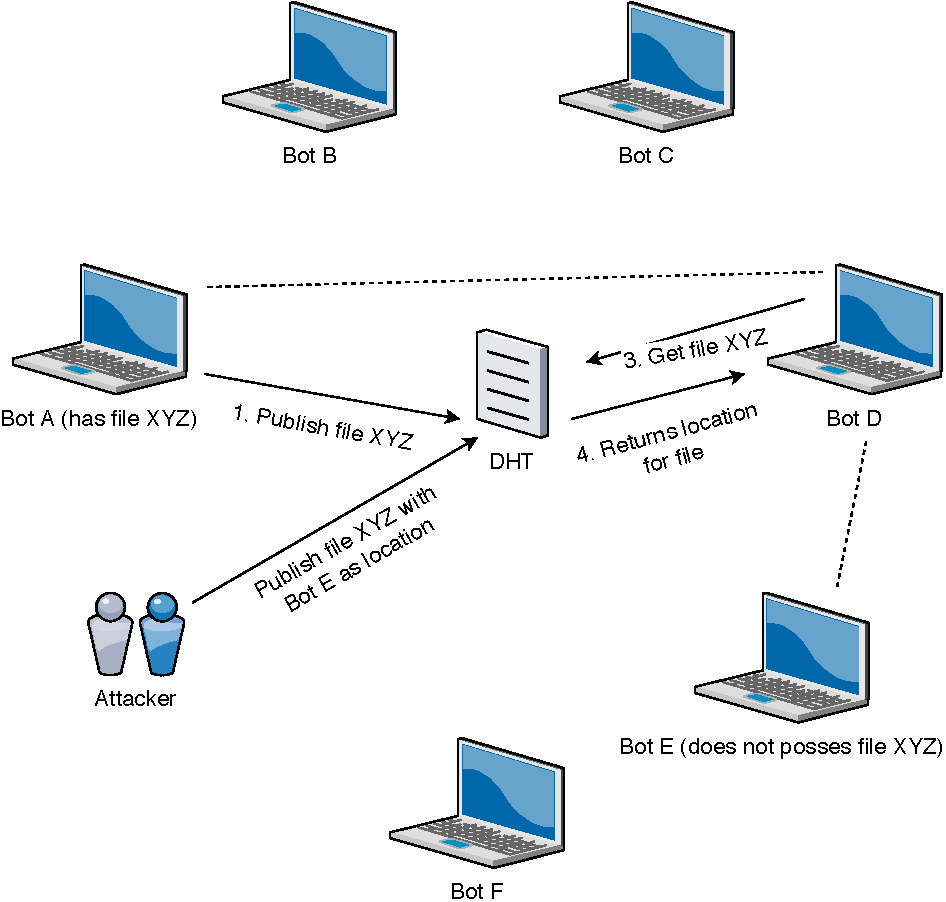
\includegraphics[width=\linewidth]{figures/index}
  \caption{Basic principle of an index poisoning attack. The attacker inserts another location into the index so that any bot who queries it will not be able to locate the requested file and instead has to lookup another location. The DHT is distributed over all bots in the network and not a central structure. The 5. step is that Bot D tries to download from one of the two provided Bots. In the case of Bot E, it will fail to fetch the file, while succeed with Bot A, thereby reducing the effectiveness. Step 5 has been excluded from the graphic for better readability.}
  \label{indexpoison}
\end{figure} 
On the other hand, the requirement for this attack is that the network is structured and the DHT does not validate the locations of newly advertised files.  
\subsection{Mitigation}\label{sybil}
The difference between \textit{Manipulation} and \textit{Mitigation} is subtle. Both are focused on slowing down a botnet, however, Mitigation does not make use of the communication protocol. Examples can be methods like a temporary Denial of Service attack against a command and control server, or a Sybil attack. 

\begin{description}
\item[Sybil:] The Sybil attack is a technique in which an attacker joins the network multiple times, however, pretends each time to be someone else. Furthermore, the attacker usually injects them as distributed as possible\cite{enisa} to have the most impact. In addition, the injected Sybil nodes have to stay active and continue to advertise themselves to the other participants. The attacker can then, for example, change the routing between the bots(like always route traffic over other Sybil nodes) and thus slow down the network. A Sybil attack can also be used to spy on the network, as \citet{sybil-crawl} have shown. \citet{sybil} did evaluate the use of a Sybil attack against the Storm botnet, which showed that it needs substantial and sustained attacks in order to bring down a botnet. \\
Sybil attacks can be prevented by the creator of the botnet by implementing the proof of work concept, as in the bitcoin P2P network. For a better understanding of the Sybil method, I have provided Figure 10, which shows a simplified P2P network in which an attacker has injected a large number of Sybil nodes.
\end{description}
\begin{figure}[ht]
  \centering
  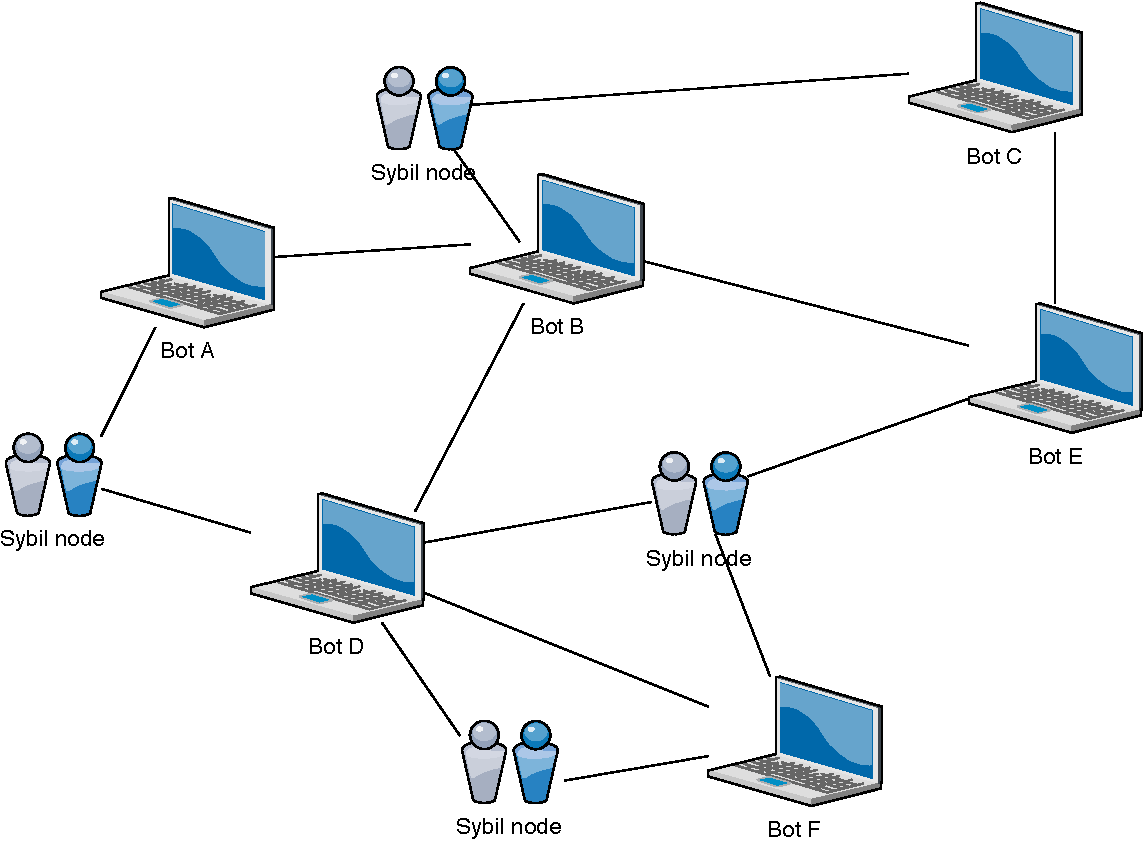
\includegraphics[width=\linewidth]{figures/sybil}
  \caption{A network invaded by sybil nodes, allowing the attacker to aquire control over the network. }
  \label{sybilfig}
\end{figure} 

\begin{description}
\item[Eclipse:] An Eclipse attack is the strategy to fully invade one specific bot's peerlist, so that the bot cannot communicate with the rest of the network. This will render the bot in the state it was at the moment of the attack, as it no longer receives any updates or new commands. An application could be, that after a successful analysis of the botnet, certain hotspots would get fully eclipsed from the network, therefore leaving the bot herder without control until he uses a new node to insert commands into the botnet. It should be noted, that this method requires not only a lot of knowledge about the topology of the network, but also of the peer-exchange algorithm used. As noted in the previous section about the resiliency of botnets, modern botnets spend a high amount of effort and time to deny the possibility of a controlled invasion of a bot's peerlist. As with the Sybil explanation, I have again provided a graphic which shows the basic concept of the eclipse attack.

\end{description}
\begin{figure}[ht]
  \centering
  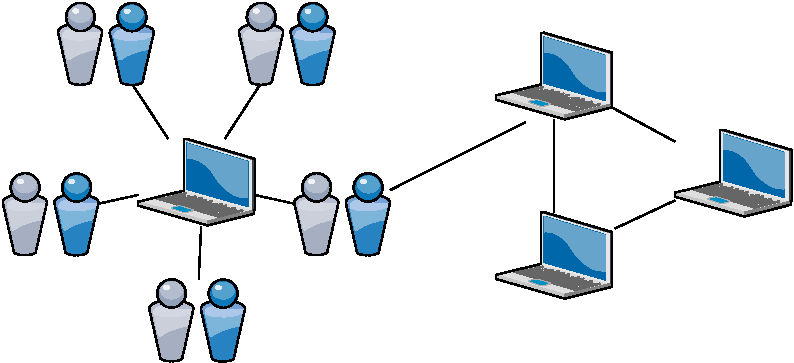
\includegraphics[width=\linewidth]{figures/eclipse}
  \caption{A bot which is fully encapsulated by nodes, which are controlled by the attacker. The bot therefore cannot gain access to communication with the rest of the network.}
  \label{eclipsefig}
\end{figure} 

Of course, there are more attacks possible than the two I have described. For instance, the partitioning attack, or the sinkhole, explained in the previous section about disruption resilience, would also be categorized as mitigation techniques. 
\subsection{Exploitation}\label{exploit}
Lastly, the category exploitation categorizes strategies and techniques which exploit the mistakes of the bot herder or the creator of the bot's software. For instance, some botnets include the functionality in their bots to uninstall themselves, when they detect that they are being run in a fake environment, like a sandbox or a virtual machine. If we could trigger this method on every bot, regardless of whether or not it is run inside a sandbox, then the whole botnet would be taken down, as the participating bots would stop to exist. But not only this can be exploited, just like bugs in normal products, we can also analyze the bots software for other vulnerabilities and use these to stop the bot. Moreover, misconfigurations can too lead to the same result.\\

Of course, this strategy is associated with a high risk since exploits can easily crash and/or damage important systems. Furthermore, they come with great problems in regard to most countries laws and raise moral questions, which are discussed in the upcoming chapter. 

\subsection{Legal and ethical problems}\label{Legislature problems}
When it comes to takedown methods and their associated legal problems, there is a lot to watch out for. Most botnets are not restricted to certain countries and instead operate all over the world---botnets do not keep to borders, so to say. As such, we lack global legislation as a legal ground for any operations to take them down. When it comes to centralized architectures, it is necessary to keep to the laws of the countries in which the command \& control server resides. In P2P networks, things start to get undefined. Which laws do apply in a network, which has no central point and instead operates worldwide? \\\\
Even when we opt for non-offensive options like sinkholing, we still need to watch out for not doing something potentially illegal. As I have noted when discussing the sinkholing technique, it comes with the problem of dealing with sensitive data. If the sinkholing happens in states of the European Union, it means that there is the need to comply with the GDPR. Moreover, when the takedown is performed by private entities, they risk rendering the evidence useless, as it not only falsifies it, it is sometimes even illegally obtained. Some states, like the Netherlands and Germany, have put laws in place, which allow the use of illegally obtained evidence when it is handed over to law enforcement\cite{silverpath}. This is particularly important, as even seemingly (legally) safe strategies like the poisoned fruit can mean trouble for the prosecution of the bot herder. \\\\
Using exploits to bring a botnet down is another part where trouble arises: In many countries, running code on a device without the permission of the owner is illegal. It also brings up the question who would be liable for any damages, when the device is interrupted in its normal operation? \\\\
Blocking the connection to command \& control servers or the network, for instance on the ISP level, requires the inspection and modifying of network traffic. Usually, this is not allowed without a warrant. This also brings us to the second part of this section: the moral problems that arise, when we take a botnet down.\\\\
We cannot rely on the end-user in order to mitigate botnets, as most do not have the required knowledge or skills to clean their infected machines. Often the end-user does also just not notice that his toaster is now part of a global botnet. Even opting for mostly risk-free methods, like taking the command \& control server offline by a Denial of Service attack, might lead to other, uninvolved parties suffering from the consequences, such as those who host their server at the same place as the bot herder. The inspection of network traffic at ISP level would be a good way to take a botnet down, yet exactly this infrastructure can be abused for censoring purposes. Taking over control over a device to fix it also bypasses the control of the owner, even though it sounds absurd that one would like their device to continue being part of a botnet. \\\\
For further input on these ethical questions in regard of doing research in the field of botnet mitigation, I will refer the interested reader to ``A Case Study in Ethical Decision Making Regarding Remote Mitigation of Botnets''\cite{ethical} by \citeauthor{ethical}.

\section{Closing remarks}
\begin{figure}[ht]
  \centering
  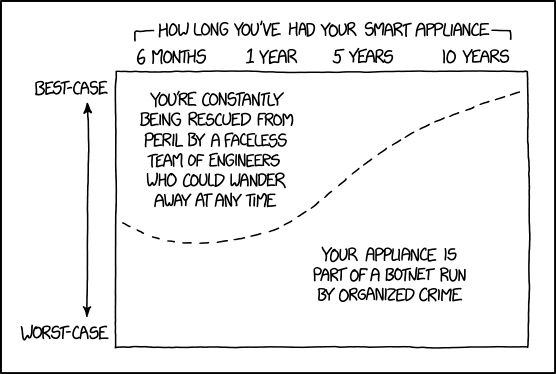
\includegraphics[width=\linewidth]{figures/xkcd}
  \caption{Credits go to xkcd\cite{xkcd} for creating this comic. Hover text: ``If they're getting valuable enough stuff from you, at least the organized crime folks have an incentive to issue regular updates to keep the appliance working after the manufacturer discontinues support.''}
  \label{xkcd}
\end{figure} 
In this paper, I gave a few examples how botnets still pose a problem, presented an overview about the architecture of botnets and their general characteristics, what we can do against them and what the risks are when it comes to newer, offensive methods. \\\\

To sum up: The threat of botnets continues to exist and their advancements in regard to resilient designs will make it harder to take them down. As more and more day to day devices are getting access to the internet as part of the internet of Things, the possible attack vectors for potential botnets are getting progressively more. The ongoing trend of automation and data exchange in manufacturing technologies also contributes to this, as it allows for blackmailing companies with their critical infrastructure. \\\\

However, recent developments, like the poisoned fruit concept promise to be a good way for low risk associated defense methods. Additionally,  methods like exploiting bugs found in the software will not disappear in the near time, thus still leaving options against highly resilient botnets, when everything else fails. 


\printbibliography[title={Bibliography}] % Print the bibliography, section title in curly brackets

\listoffigures
%----------------------------------------------------------------------------------------

\end{document}
